\documentclass{article}%
\usepackage[T1]{fontenc}%
\usepackage[utf8]{inputenc}%
\usepackage{lmodern}%
\usepackage{textcomp}%
\usepackage{lastpage}%
\usepackage[tmargin=1cm,bmargin=2cm,lmargin=1cm]{geometry}%
\usepackage{multicol}%
\usepackage{graphicx}%
\usepackage{adjustbox}%
\usepackage{tkz-euclide}%
\usepackage{amsmath}%
\usepackage{scalefnt}%
\usepackage{enumitem}%
%
%
%
\begin{document}%
\normalsize%
\setlength\itemsep{-2cm}%
\section{Identifying the four types of slope}%
\label{sec:Identifyingthefourtypesofslope}%
\textbf{Learning Goal: }\hrulefill \\ \hrulefill%
\begin{multicols}{2}%
\begin{enumerate}[label=\arabic*),start=1]%
\item\adjustbox{valign=t}{\begin{minipage}{\linewidth}
Find the slope of each line segment. For each type of slope, list the segments that have that type of slope.\\

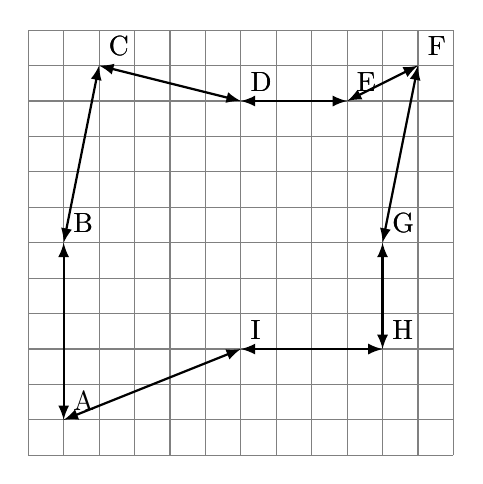
\begin{tikzpicture}[scale=0.45]
   \tkzInit[xmax=6,ymax=6,xmin=-6,ymin=-6]
   \tkzGrid
   \tkzAxeXY
    
        \node[anchor=south west](p000) at (-5,-5){ A };
        \node[anchor=south west](p000) at (-5,0){ B };
        \draw[ thick,latex-latex] (-5,-5) -- (-5,0);% node[anchor=south west] {$['A', 'B']$}; % two points for drawing 2x+y=2
    
        \node[anchor=south west](p100) at (-5,0){ B };
        \node[anchor=south west](p100) at (-4,5){ C };
        \draw[ thick,latex-latex] (-5,0) -- (-4,5);% node[anchor=south west] {$['B', 'C']$}; % two points for drawing 2x+y=2
    
        \node[anchor=south west](p200) at (-4,5){ C };
        \node[anchor=south west](p200) at (0,4){ D };
        \draw[ thick,latex-latex] (-4,5) -- (0,4);% node[anchor=south west] {$['C', 'D']$}; % two points for drawing 2x+y=2
    
        \node[anchor=south west](p300) at (0,4){ D };
        \node[anchor=south west](p300) at (3,4){ E };
        \draw[ thick,latex-latex] (0,4) -- (3,4);% node[anchor=south west] {$['D', 'E']$}; % two points for drawing 2x+y=2
    
        \node[anchor=south west](p400) at (3,4){ E };
        \node[anchor=south west](p400) at (5,5){ F };
        \draw[ thick,latex-latex] (3,4) -- (5,5);% node[anchor=south west] {$['E', 'F']$}; % two points for drawing 2x+y=2
    
        \node[anchor=south west](p500) at (5,5){ F };
        \node[anchor=south west](p500) at (4,0){ G };
        \draw[ thick,latex-latex] (5,5) -- (4,0);% node[anchor=south west] {$['F', 'G']$}; % two points for drawing 2x+y=2
    
        \node[anchor=south west](p600) at (4,0){ G };
        \node[anchor=south west](p600) at (4,-3){ H };
        \draw[ thick,latex-latex] (4,0) -- (4,-3);% node[anchor=south west] {$['G', 'H']$}; % two points for drawing 2x+y=2
    
        \node[anchor=south west](p700) at (4,-3){ H };
        \node[anchor=south west](p700) at (0,-3){ I };
        \draw[ thick,latex-latex] (4,-3) -- (0,-3);% node[anchor=south west] {$['H', 'I']$}; % two points for drawing 2x+y=2
    
        \node[anchor=south west](p800) at (0,-3){ I };
        \node[anchor=south west](p800) at (-5,-5){  };
        \draw[ thick,latex-latex] (0,-3) -- (-5,-5);% node[anchor=south west] {$['I', '']$}; % two points for drawing 2x+y=2
    
  \end{tikzpicture}
\end{minipage}}%
\begin{enumerate}[label=\alph*)]%
\item positive: \hrulefill%
\item negative: \hrulefill%
\item 0: \hrulefill%
\item undefined: \hrulefill%
\end{enumerate}%
\vspace{0cm}%
\item\adjustbox{valign=t}{\begin{minipage}{\linewidth}
Graph the equation $y=\frac{3}{2}x$. Is the slope positive, negative, zero, or undefined?\\

%\vspace{4cm}

\begin{tikzpicture}[font=\small,scale=0.40]
   \tikzstyle{every node}=[font=\small]
   \tkzInit[xmax=6,ymax=6,xmin=-6,ymin=-6]
   \tkzGrid
   \tkzAxeXY
%   \draw[ thick,latex-latex] (-1,4) -- (4,-6) node[anchor=south west] {$a$}; % two points for drawing 2x+y=2
%  \tkzText[above](0,6.75){Desired Output}
  \end{tikzpicture}
\end{minipage}}%
\vspace{0cm}%
\item\adjustbox{valign=t}{\begin{minipage}{\linewidth}
What is the slope of the graph below?\\

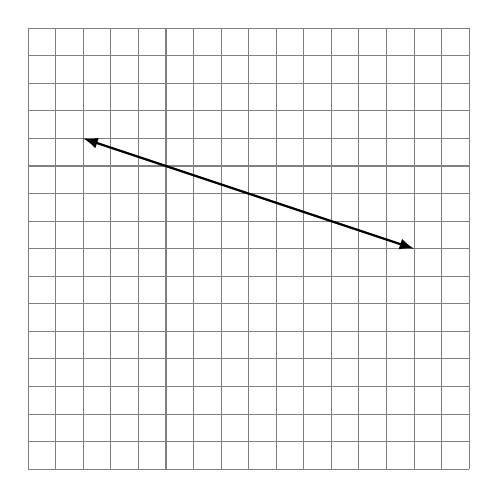
\begin{tikzpicture}[font=\tiny,scale=0.35]
   %\tikzstyle{every node}=[font=\small]
   \tkzInit[xmax=8,ymax=8,xmin=-8,ymin=-8]
   \tkzGrid
   \tkzAxeXY
   \draw[ thick,latex-latex] (-6,4) -- (6,0);% node[anchor=south west] {$a$}; % two points for drawing 2x+y=2
%  \tkzText[above](0,6.75){Desired Output}
  \end{tikzpicture}
\end{minipage}}%
\vspace{0cm}%
\item\adjustbox{valign=t}{\begin{minipage}{\linewidth}
Match each line with the description of its slope\\

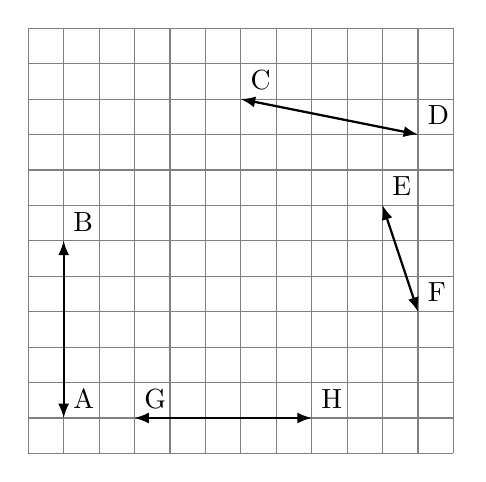
\begin{tikzpicture}[scale=0.45]
   \tkzInit[xmax=6,ymax=6,xmin=-6,ymin=-6]
   \tkzGrid
   \tkzAxeXY
    
        \node[anchor=south west](p000) at (-5,-5){ A };
        \node[anchor=south west](p000) at (-5,0){ B };
        \draw[ thick,latex-latex] (-5,-5) -- (-5,0);% node[anchor=south west] {$['A', 'B']$}; % two points for drawing 2x+y=2
    
        \node[anchor=south west](p100) at (0,4){ C };
        \node[anchor=south west](p100) at (5,3){ D };
        \draw[ thick,latex-latex] (0,4) -- (5,3);% node[anchor=south west] {$['C', 'D']$}; % two points for drawing 2x+y=2
    
        \node[anchor=south west](p200) at (4,1){ E };
        \node[anchor=south west](p200) at (5,-2){ F };
        \draw[ thick,latex-latex] (4,1) -- (5,-2);% node[anchor=south west] {$['E', 'F']$}; % two points for drawing 2x+y=2
    
        \node[anchor=south west](p300) at (-3,-5){ G };
        \node[anchor=south west](p300) at (2,-5){ H };
        \draw[ thick,latex-latex] (-3,-5) -- (2,-5);% node[anchor=south west] {$['G', 'H']$}; % two points for drawing 2x+y=2
    
  \end{tikzpicture}
\end{minipage}}%
\begin{enumerate}[label=\alph*)]%
\item \overline{AB} \hfill positive%
\item \overline{CD} \hfill negative%
\item \overline{EF} \hfill zero%
\item \overline{GH} \hfill undefined%
\end{enumerate}%
\vspace{0cm}%
\item\adjustbox{valign=t}{\begin{minipage}{\linewidth}
Graph the equation $y=-\frac{1}{2}x$. Is the slope positive, negative, zero, or undefined?\\

%\vspace{4cm}

\begin{tikzpicture}[font=\small,scale=0.40]
   \tikzstyle{every node}=[font=\small]
   \tkzInit[xmax=6,ymax=6,xmin=-6,ymin=-6]
   \tkzGrid
   \tkzAxeXY
%   \draw[ thick,latex-latex] (-1,4) -- (4,-6) node[anchor=south west] {$a$}; % two points for drawing 2x+y=2
%  \tkzText[above](0,6.75){Desired Output}
  \end{tikzpicture}
\end{minipage}}%
\vspace{0cm}%
\item\adjustbox{valign=t}{\begin{minipage}{\linewidth}
What is the rate of change of the relationship in represented by the table?\\

    \begin{tabular}{ | c | c |}
    \hline
    x & y \\ \hline
    
        -4 & 0 \\
    
        -2 & 1 \\
    
        0 & 2 \\
    
    \hline
    \end{tabular}
\end{minipage}}%
\vspace{0cm}%
\item\adjustbox{valign=t}{\begin{minipage}{\linewidth}
What is the slope of the line through the points $(-1,7)$ and $(3,-9)$?\\

\end{minipage}}%
\vspace{1.75cm}%
\item\adjustbox{valign=t}{\begin{minipage}{\linewidth}
What is the rate of change of the relationship in represented by the table?\\

    \begin{tabular}{ | c | c |}
    \hline
    x & y \\ \hline
    
        -5 & 1 \\
    
        -3 & 4 \\
    
        1 & 10 \\
    
    \hline
    \end{tabular}
\end{minipage}}%
\vspace{0cm}%
\item\adjustbox{valign=t}{\begin{minipage}{\linewidth}
What is the slope of the line through the points $(-2,5)$ and $(5,-5)$?\\

\end{minipage}}%
\vspace{1.75cm}%
\item\adjustbox{valign=t}{\begin{minipage}{\linewidth}
Find the slope of each line segment. For each type of slope, list the segments that have that type of slope.\\

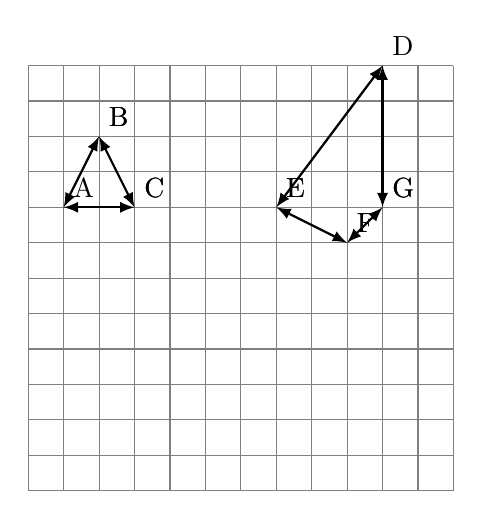
\begin{tikzpicture}[scale=0.45]
   \tkzInit[xmax=6,ymax=6,xmin=-6,ymin=-6]
   \tkzGrid
   \tkzAxeXY
    
        \node[anchor=south west](p000) at (-5,2){ A };
        \node[anchor=south west](p000) at (-4,4){ B };
        \draw[ thick,latex-latex] (-5,2) -- (-4,4);% node[anchor=south west] {$['A', 'B']$}; % two points for drawing 2x+y=2
    
        \node[anchor=south west](p100) at (-4,4){ B };
        \node[anchor=south west](p100) at (-3,2){ C };
        \draw[ thick,latex-latex] (-4,4) -- (-3,2);% node[anchor=south west] {$['B', 'C']$}; % two points for drawing 2x+y=2
    
        \node[anchor=south west](p200) at (-3,2){ C };
        \node[anchor=south west](p200) at (-5,2){  };
        \draw[ thick,latex-latex] (-3,2) -- (-5,2);% node[anchor=south west] {$['C', '']$}; % two points for drawing 2x+y=2
    
        \node[anchor=south west](p300) at (4,6){ D };
        \node[anchor=south west](p300) at (1,2){ E };
        \draw[ thick,latex-latex] (4,6) -- (1,2);% node[anchor=south west] {$['D', 'E']$}; % two points for drawing 2x+y=2
    
        \node[anchor=south west](p400) at (1,2){ E };
        \node[anchor=south west](p400) at (3,1){ F };
        \draw[ thick,latex-latex] (1,2) -- (3,1);% node[anchor=south west] {$['E', 'F']$}; % two points for drawing 2x+y=2
    
        \node[anchor=south west](p500) at (3,1){ F };
        \node[anchor=south west](p500) at (4,2){ G };
        \draw[ thick,latex-latex] (3,1) -- (4,2);% node[anchor=south west] {$['F', 'G']$}; % two points for drawing 2x+y=2
    
        \node[anchor=south west](p600) at (4,2){ G };
        \node[anchor=south west](p600) at (4,6){  };
        \draw[ thick,latex-latex] (4,2) -- (4,6);% node[anchor=south west] {$['G', '']$}; % two points for drawing 2x+y=2
    
  \end{tikzpicture}
\end{minipage}}%
\begin{enumerate}[label=\alph*)]%
\item positive: \hrulefill%
\item negative: \hrulefill%
\item 0: \hrulefill%
\item undefined: \hrulefill%
\end{enumerate}%
\vspace{0cm}%
\item\adjustbox{valign=t}{\begin{minipage}{\linewidth}
Graph the equation $y=3x$. Is the slope positive, negative, zero, or undefined?\\

%\vspace{4cm}

\begin{tikzpicture}[font=\small,scale=0.40]
   \tikzstyle{every node}=[font=\small]
   \tkzInit[xmax=6,ymax=6,xmin=-6,ymin=-6]
   \tkzGrid
   \tkzAxeXY
%   \draw[ thick,latex-latex] (-1,4) -- (4,-6) node[anchor=south west] {$a$}; % two points for drawing 2x+y=2
%  \tkzText[above](0,6.75){Desired Output}
  \end{tikzpicture}
\end{minipage}}%
\vspace{0cm}%
\item\adjustbox{valign=t}{\begin{minipage}{\linewidth}
Graph the equation $y=-5x$. Is the slope positive, negative, zero, or undefined?\\

%\vspace{4cm}

\begin{tikzpicture}[font=\small,scale=0.40]
   \tikzstyle{every node}=[font=\small]
   \tkzInit[xmax=6,ymax=6,xmin=-6,ymin=-6]
   \tkzGrid
   \tkzAxeXY
%   \draw[ thick,latex-latex] (-1,4) -- (4,-6) node[anchor=south west] {$a$}; % two points for drawing 2x+y=2
%  \tkzText[above](0,6.75){Desired Output}
  \end{tikzpicture}
\end{minipage}}%
\vspace{0cm}%
\end{enumerate}

%
\end{multicols}%
\end{document}